The algorithm was initially applied to all the DT chambers of the barrel. However the
illumation of the chambers by cosmic tracks, crossing also the central sillicon tracker,
was irregular and in many cases insufficient due to the topology of cosmic tracks. The number
of global tracks collected in the DT chambers covering a $abs(\eta)>0.5$ range did not allow
to perform a good alignment of the chambers in the most external wheels $2$ and $-2$. This was
the case also of the sectors $1$ and $7$ whom planes are orthogonal to the ground. The illumination
received by these chambers was also small as the number of cosmic tracks parallel to the ground is
small. For this reason, these chambers were not either aligned. In addition chambers in wheel
$-1$, station $2$, sector $8$ and wheel $1$, station $3$ and sector $8$ were neither aligned
because of problems in the convergency of the fit.

In figure \ref{resultsMillepede} the measured alignment parameters with respect to the nominal
geometry are shown.   

\begin{figure}[h!]
  \centering
  \subfigure[]{
    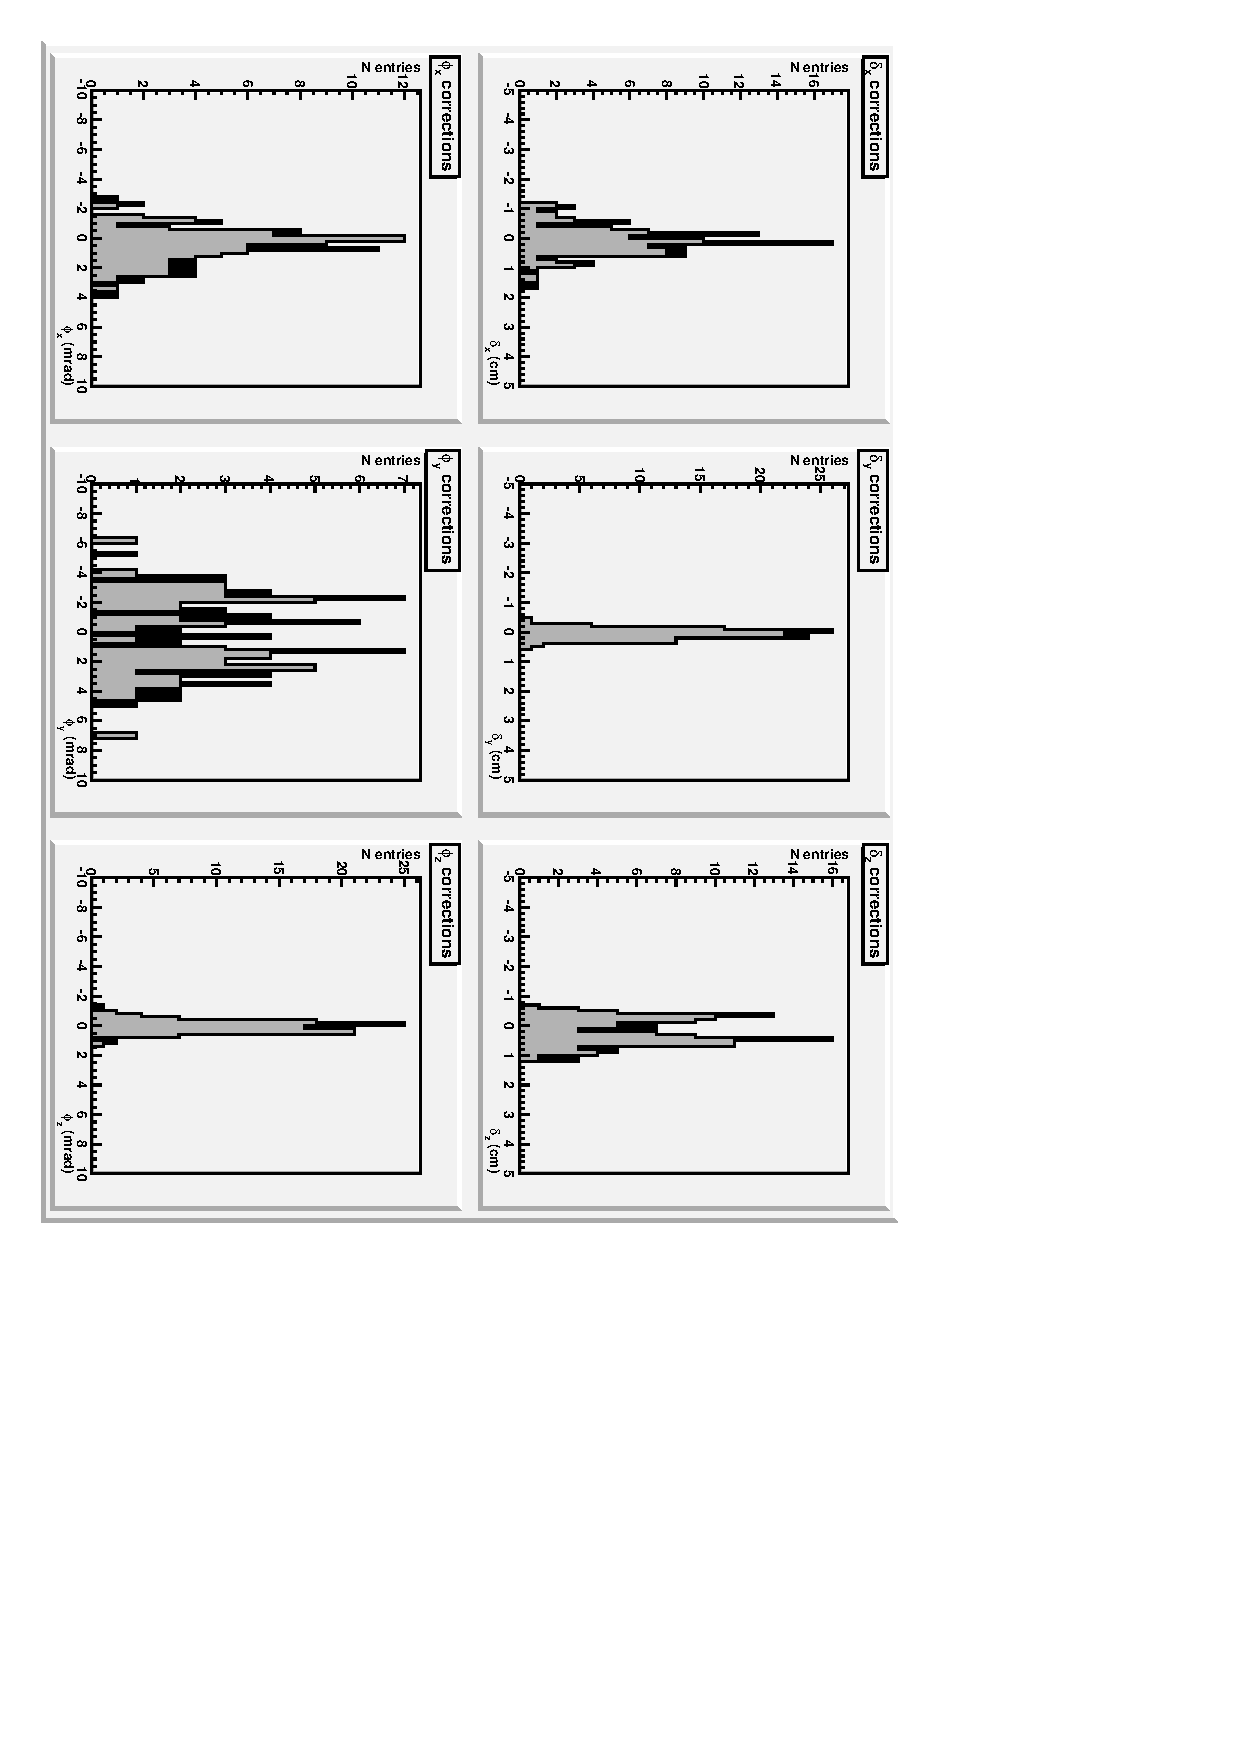
\includegraphics[width=0.7\textwidth, angle=90]{plots/gma_mp_results/MillepedeResults.pdf}
  }
  \label{resultsMillepede}
  \caption{Values of the alignment parameters as measured by the Millepede algorithm} 
\end{figure}
 
